%! Author = Len Washington III
%! Date = 8/12/2023

% Preamble
\documentclass[2]{cs430homework}

% Document
\begin{document}

\maketitle

\begin{enumerate}[label=\arabic*.]
	\item (5 points) We have a problem that can be solved by an iterative (non-recursive) algorithm that operates in $N^{2}$ time. We also have a recursive algorithm for this problem that takes $N \lg N$ operations to divide the input into two equal pieces, two recursive calls to conquer, and $\lg N$ operations to combine the two solutions together. Show whether the iterative or recursive version is more efficient.
	\item (6 points) During the running of the procedure RANDOMIZED-QUICKSORT, how many calls are made to the random-number generator RANDOM in the worst case? How about in the best case? Give your answer in terms of $\Theta$-notation.\begin{algorithm}[H]
		\caption{Randomized-Partition pulled from the book.}\label{alg:randomized-partition}
		\begin{algorithmic}[1]
		\Function{Randomized-Partition}{$A$, $p$, $r$}
			\State $i \gets$ \Call{Random}{$p$, $r$}
			\State exchange $A$[$r$] with $A$[$i$]
			\State \Return \Call{Partition}{$A$, $p$, $r$}
		\EndFunction
		\end{algorithmic}
	\end{algorithm}\begin{algorithm}[H]
			\caption{Randomized-Quicksort pulled from the book.}\label{alg:randomized-quicksort}
			\begin{algorithmic}[1]
			\Function{Randomized-Quicksort}{$A$, $p$, $r$}
				\If{$p < r$}
					\State $q \gets $ \Call{Randomized-Partition}{$A$, $p$, $r$}
					\State \Call{Randomized-Quicksort}{$A$, $p$, $q-1$}
					\State \Call{Randomized-Quicksort}{$A$, $q+1$, $r$}
				\EndIf
			\EndFunction
			\end{algorithmic}
		\end{algorithm}
	\item (5 points) Give pseudocode, code or a description of an algorithm to rearrange the objects in array so that the objects with odd number keys come first (in any order, not necessarily sorted), followed by the objects with even numbers (also any order), returning the position of the first even number object. What is the big-O runtime of your algorithm? \\
	So, for example, $\left\{1,0,8,7,5,3,9,6,2,7,4\right\}$ might become $\left\{1,7,9,7,5,3,8,6,2,0,4\right\}$ and the index 7 (the new position of value 8) is returned.
	\item Suppose you are given $k$ $n$-element sorted sequences $A_{i}$. Each sequence has no duplicate entries, but there may be duplicates between sequences. Describe an $O(nk \log k)$-time method that uses a minheap for computing a sorted sequence representing the union of all $A_{i}$ sequences, with no duplicates. Discuss why your algorithm is $O(nk \log k)$.
	\item This problem requires you to use a heap to store items, but instead of using a key of an item to determine where to store the item in the heap, you need to assign a priority (key) to each item that will determine where it is inserted in the heap
	\begin{enumerate}[label=\arabic{enumi}\alph*)]
	    \item (4 points) Show how to assign priorities to items to implement a first-in, first-out queue with a heap.
		\item (4 points) Show how to assign priorities to items to implement a first-in, last-out stack with a heap.
	\end{enumerate}
	\item (6 points) Show that the second smallest of $n$ elements can be found with $(n-1) + (\lceil \lg n \rceil-1)$ comparisons in the worst case. Use a tournament (upside down binary tree) approach to also find the smallest element and think about where the second-smallest element might be in the tournament. Hint: The number of comparisons shown above is shown as two terms because there are two steps to the algorithm.
	\item (4 points) The following comparison tree sorts the four values a, b, c, and d.
	\begin{figure}[H]
		\centering
		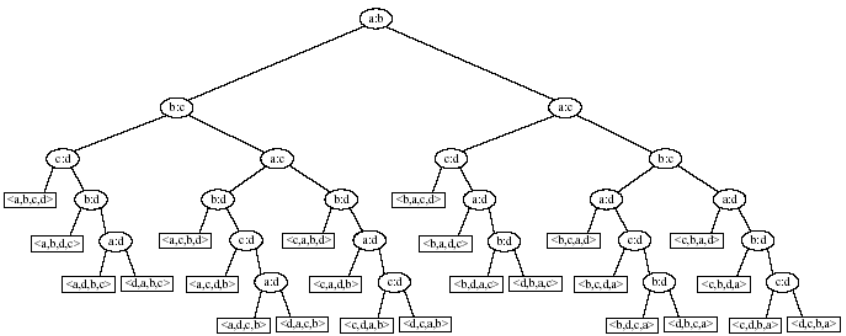
\includegraphics[width=1.1\textwidth]{2.7}
		\caption{}
		\label{fig:2.7}
	\end{figure}
	\begin{enumerate}[label=\arabic{enumi}\alph*)]
		\item What is the worst-case number of comparisons performed by the comparison tree?
		\item What is the best-case number of comparisons performed by the comparison tree?
		\item What is the average-case number of comparisons performed by the comparison tree, assuming that any permutation of the four inputs is equally likely?
	\end{enumerate}
\end{enumerate}

% TODO: 1, 7c, 4, 5b

\end{document}